\documentclass[tikz,border=6pt]{standalone}
\usepackage{fontspec}
\setmainfont{Noto Sans}
\usepackage{amsmath,amssymb}
\usepackage{tikz}
\usetikzlibrary{arrows.meta,positioning,calc}
\definecolor{cudaG}{RGB}{118,185,0}
\definecolor{gsBlue}{RGB}{40,110,190}
\definecolor{bgGray}{RGB}{242,242,242}
\begin{document}
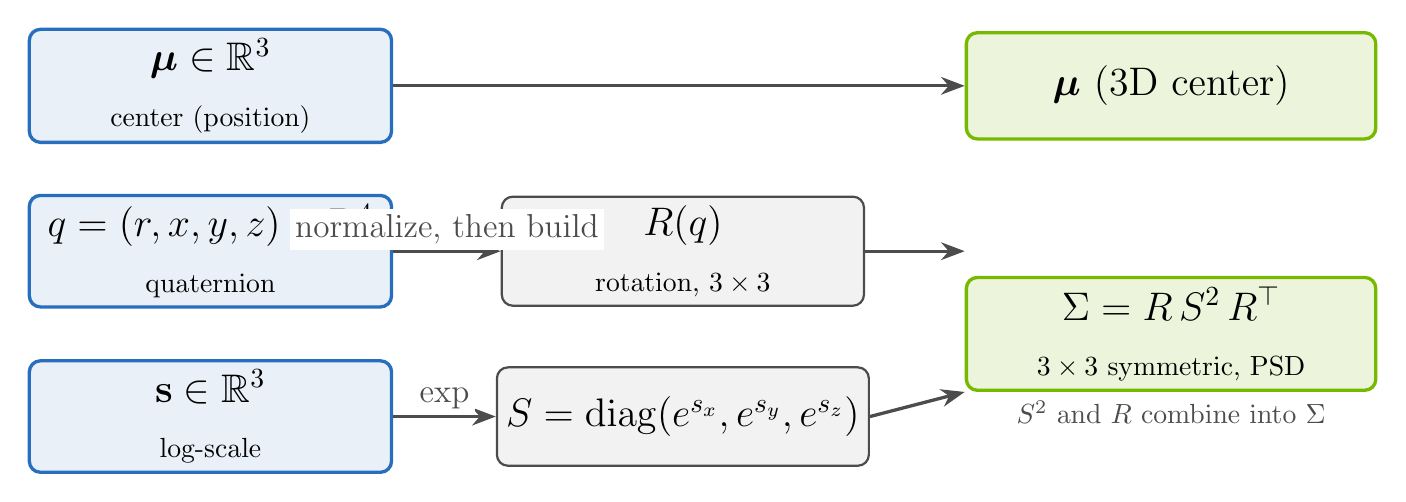
\begin{tikzpicture}[
  inp/.style={draw=gsBlue, very thick, rounded corners, fill=gsBlue!10, minimum width=4.6cm, minimum height=1.25cm, align=center, font=\Large},
  proc/.style={draw=black!70, thick, rounded corners, fill=bgGray, minimum width=4.6cm, minimum height=1.25cm, align=center, font=\Large},
  outb/.style={draw=cudaG, very thick, rounded corners, fill=cudaG!14, minimum width=5.2cm, minimum height=1.35cm, align=center, font=\Large},
  arr/.style={-{Stealth[length=3mm]}, very thick, black!70},
  lab/.style={font=\large, text=black!70, fill=white, inner sep=2pt}
]
  % inputs (left column)
  \node[inp] (mu) at (0,4.2) {$\boldsymbol{\mu}\in\mathbb{R}^3$\\[2pt]{\normalsize center (position)}};
  \node[inp] (q)  at (0,2.1) {$q=(r,x,y,z)\in\mathbb{R}^4$\\[2pt]{\normalsize quaternion}};
  \node[inp] (s)  at (0,0)   {$\mathbf{s}\in\mathbb{R}^3$\\[2pt]{\normalsize log-scale}};

  % processing (middle column)
  \node[proc] (R) at (6,2.1) {$R(q)$\\[2pt]{\normalsize rotation, $3\times3$}};
  \node[proc] (S) at (6,0)   {$S=\mathrm{diag}(e^{s_x},e^{s_y},e^{s_z})$};

  % output (right column)
  \node[outb] (Sig) at (12.2,1.05) {$\Sigma=R\,S^{2}\,R^{\top}$\\[2pt]{\normalsize $3\times3$ symmetric, PSD}};
  \node[outb] (mo) at (12.2,4.2) {$\boldsymbol{\mu}$ (3D center)};

  \draw[arr] (q) -- node[lab,above] {normalize, then build} (R);
  \draw[arr] (s) -- node[lab,above] {$\exp$} (S);
  \draw[arr] (R) -- (Sig.west |- R) ;
  \draw[arr] (S.east) -- (Sig.south west);
  \draw[arr] (mu) -- (mo);
  \node[lab,below=1pt of Sig, font=\normalsize] {$S^2$ and $R$ combine into $\Sigma$};
\end{tikzpicture}
\end{document}
